\documentclass[11pt, a4paper]{article}
\usepackage[utf8]{inputenc}
\usepackage[T1]{fontenc}
\usepackage[margin=1in, left=0.5in, right=1in]{geometry}
\usepackage{graphicx}
\usepackage{enumitem}
\usepackage{xcolor}
\usepackage{hyperref}
\usepackage{fancyhdr}
\usepackage{cite}
\usepackage[scaled]{helvet}
\renewcommand{\familydefault}{\sfdefault} % Set the default font to Sans-Serif
\usepackage[T1]{fontenc}
\usepackage{float}
% \usepackage{minted}


% Define TUM Blue
\definecolor{tumblue}{RGB}{0, 101, 189}

\pagestyle{empty}

\begin{document}

% --- Header: Two Column Layout using Minipages ---
\begin{flushright}
    
\includegraphics[width=0.1\textwidth]{img/TUM_logo.png}
\end{flushright}

\noindent
\begin{minipage}[t]{0.75\textwidth}
    \vspace{0pt}
    {\Large \textbf{Vulnerability Patching via Structure-Aware Retrieval-Augmented Generation}} \\
    \large \textcolor{gray}{Master's Thesis}
    
    \vspace{0.8cm}
    \centering
    \small
    \begin{tabular}{@{}ll}
       \textbf{Supervisor:}   & Prof. Dr. Jana Giceva Makreshanska \\
        \textbf{Advisor:}      & Fabian Wenz \\
        \textbf{Email:}        & \texttt{jana.giceva@in.tum.de} \\
        \textbf{Phone:}        & +49 (0) 89 / 289-17286 \\
        \textbf{Starting date:} & April 2026 \\
    \end{tabular}
\end{minipage}
\begin{minipage}[t]{0.25\textwidth}
    \vspace{0pt}
    \begin{flushright}
        
        \scriptsize
        \scriptsize
        \textbf{TUM School of Computation, \\ Information and Technology} \\[0.2cm]
        Institut für Informatik \\
        Lehrstuhl III (I3) \\
        Prof. Dr. Jana Giceva Makreshanska \\[0.2cm]
        Boltzmannstr. 3 \\
        Room: 02.11.043 \\
        85748 Garching \\[0.2cm]
        \url{https://www.db.in.tum.de/}
    \end{flushright}
\end{minipage}

\vspace{1cm}
\vspace{0.8cm}
% --- Body Content ---
\section*{Context}
\subsection{Research Background}
To meet compliance requirements, organizations must adhere to International Standards and regulations such as ISO/IEC 27001 \cite{iso27001}. This standard establishes best practices for data protection, cyber-resilience, and operational excellence. 
To accomplish that and improve development robustness, enterprises must anticipate and adapt to vulnerabilities and potential attacks. 
For software companies, this goal demands evolving software development life cycles to rapidly identify, generate, and deploy risk mitigation for vulnerabilities. 
One possible approach is to integrate automated systems that proactively generate patches for buggy programs. 

With the advent and widespread adoption of Large Language Models (LLMs), a new venue for automated remediation emerged \cite{Xia_2024}. 
However, the current LLM approaches remain insufficient for security patching due to two primary failure reasons:

\begin{enumerate}[leftmargin=*, label=\arabic*.]

    \item \textbf{Semantic Misunderstanding:} 84–94\% of AI patches rely on localized fixes that fail to address root causes, making them significantly more fragile and easier to bypass than human-authored patches \cite{mahmud2025systematic}.

    \item \textbf{Vulnerability Identification Failures:} Models frequently misidentify vulnerability contexts, with some retrieval tasks showing failure rates as high as 91.6\% \cite{McClanahan2024Meets}. 
    This leads to "semantic hallucinations", where a model might apply mitigation steps for the wrong operating system \cite{McClanahan2024Meets} or package version \cite{zemicheal2024llm}, creating a false sense of security while leaving the actual system exposed.

\end{enumerate}

\subsection{Problem Statement}
These failures are aggravated by providing lengthy raw source code to the LLM. 
In these cases, vulnerability-relevant logic is diluted by implementation details and boilerplate code, thereby degrading the quality of security analysis \cite{contextenhancedYang}.
Empirical results from the same work suggest that this code noise induces what the authors term Analysis Focus Drift, wherein the model performs a code quality review rather than a vulnerability analysis.
Thus, there is an opportunity to develop methodologies that enrich security-relevant information while filtering out implementation noise. 
Moreover, although various studies show that knowledge bases improve LLM responses in security applications \cite{du2025vulragenhancingllmbasedvulnerability, seo2026autopatch, wang2025valign, guo2025bluecodeagentblueteamingagent}, it is unclear which approach optimizes patch quality effectively in multi-agent environments.

This work contributes to the exploration of this gap by proposing a Retrieval-Augmented Generation (RAG) system that uses graph-based representations of code vulnerabilities to generate embeddings.

\subsection{Research Objectives}

To evaluate the proposed framework, we address two primary research questions:
 
\textbf{RQ1: }How effective are graph-based embeddings at retrieving relevant vulnerability fix patterns from the knowledge base?
 
\textbf{RQ2: }What are the trade-offs of using Graph-RAG in the vulnerability patching pipeline?

If within reach, we aim to also address the following complementary research questions:
 
\textbf{CRQ1: }How does the structure-aware RAG framework with a small model compare with existing approaches (e.g., zero-shot small models and AutoPatch)?

\textbf{CRQ2: }What is the computational and financial cost of the approach (e.g., token usage, storage complexity and size, end-to-end pipeline costs)? 

\section*{Related Work}
Automated Program Repair (APR) aims to fix functional and security defects, which are critical in large-scale software systems.
With advances in LLM coding capabilities, systems such as RepairAgent \cite{bouzenia2025repairagent} have demonstrated that autonomous LLM agents can resolve hundreds of bugs through iterative tool interaction.
However, this process comes at a high computational cost, averaging 270,000 tokens per bug, raising concerns about the efficiency of these approaches.

Automated Vulnerability Repair (AVR), a subtask of APR, focuses on addressing software security vulnerabilities while minimizing dependence on domain experts \cite{vulrepair2025usenix}.
However, APR techniques do not transfer seamlessly to AVR \cite{pinconshi2021comparativeaprvul}, necessitating specialized approaches.
Systems such as FineNib \cite{wang2026finenib} exemplify this complexity by incorporating formal static analysis artifacts, specifically CodeQL queries, as executable verification oracles during code generation. 
In contrast to approaches that rely on existing security tools, AutoPatch \cite{seo2026autopatch} proposes a system grounded through RAG and multiple agent interactions to achieve meaningful results. 
RAG was originally proposed to combine the flexibility of pre-trained parametric memory with the precision of non-parametric external knowledge \cite{lewis2020rag}, enabling models to consult a document index and reason beyond their training data.
Despite these advantages, RAG-based approaches identified in this review depend exclusively on textual vector embeddings for retrieval, failing to capture deep structural signatures of vulnerabilities, such as taint flows, data dependency chains, and control flow anomalies. 
This limitation creates a representational gap, causing these systems to fall back on the inherent capacity of the generative model, assuming that scale is the main lever for repair quality.
Consequently, this dependency results in high repair costs and structural logic errors \cite{cao2024cutting}.

Prior to the recent advancements in LLM-based code understanding \cite{llmcodeadvances}, static analysis techniques such as Code Property Graphs (CPGs) \cite{cpgyamaguchi} were already well established. 
CPG is a code representation that merges abstract syntax trees, control flow graphs, and data flow graphs into a joint data structure, facilitating vulnerability detection through graph traversal.
Although CPGs have been applied to vulnerability detection, their potential as a retrieval representation for automated vulnerability repair remains unexplored.

The proposed approach aims to ground retrieval in graph embeddings, using structural similarity as the primary retrieval signal, rather than relying only on semantic keyword matching.

\section*{Methodology}

This work proposes a structure-aware RAG framework for automated vulnerability patching.
Rather than relying only on the generative capacity of frontier models, this approach shifts part of the patching complexity to retrieval precision, better grounding the repair process.

The vulnerable code will be represented using graph embeddings to retrieve structurally similar patches from a knowledge base at inference time.
Beyond retrieval, we will apply the graph edit distance \cite{gao2010survey, li2019simgnn} to identify structural differences between vulnerable and patched code within the retrieved pairs.
These structural differences serves as a grounding repair orientation for the LLM to remediate a flaw. 

We investigated how this design leverages structural meaning encoded in graph representations to identify the lines that introduce security breaches.

\subsection*{Architecture }

The architecture employed in this work is displayed in \figurename{\ref{fig:sysdesign}},
where the box containing $\Delta$ represents our contribution. All the other components are derived from existing frameworks.

The system consists of a knowledge base (KB) and an agentic framework.
The KB is constructed from datasets annotated with CVE (Common Vulnerabilities and Exposures) and CWE (Common Weakness Enumeration). Each entry contains the vulnerable/patched code pair and its structural differences extracted via subgraph matching.

The system will use an agentic framework common in industrial applications and similar to the AutoPatch \cite{seo2026autopatch} design and employ two specialized LLM agents: 

\begin{itemize}
    \item Patcher Agent: synthesizes code repairs by using the retrieved context in its prompt; 
    \item Vulnerability Verifier Agent: receives the generated patch and verifies whether the previously spotted vulnerability persists.
\end{itemize}

\begin{figure}[H]
  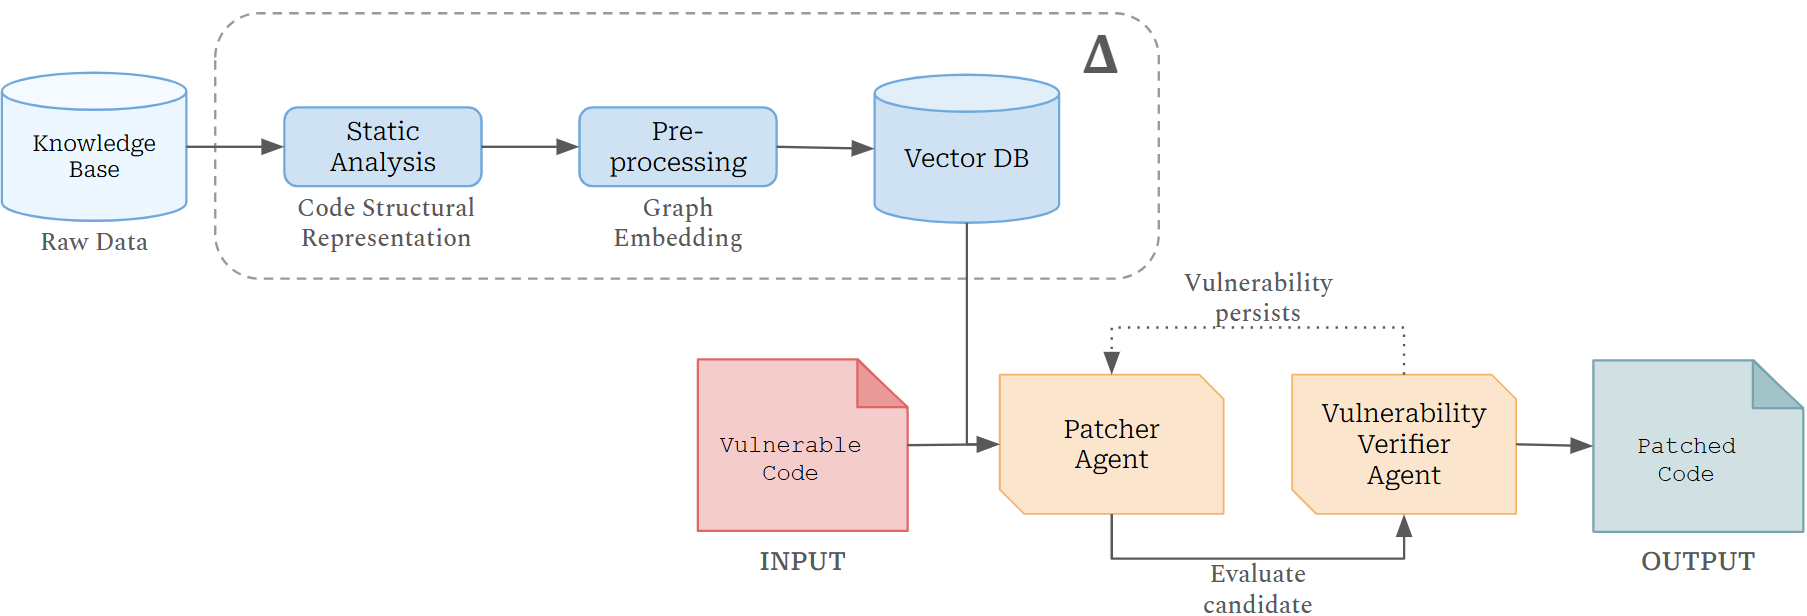
\includegraphics[width=\linewidth]{img/arch.png}
  \caption{System architecture used in this work to verify the graph embedding usage for patching vulnerabilities, where the $\Delta$-box is our contribution.}
  \label{fig:sysdesign}
\end{figure}

 \subsection*{Data Pipeline}
\subsection*{Graph Generation}
This work utilizes Joern to generate the Code Property Graph (CPG) from a code snippet. 
For snippets that are not well-formed C/C++ programs, the pipeline first wraps the code with the minimum necessary macros and type definitions (e.g. \ \verb|typedef unsigned int u32|, \verb|#define NULL ((void*)0)|) and writes a parseable source file.
The C/C++ code files are exported to a binary graph  with the Joern shell command \verb|joern-parse --language newc|, where \verb|newc| specifies the C++ specifities avoiding will-formed graphs.  
Then, the compiled graph is exported to GraphML format with the shell-command \verb|joern-export --repr cpg --format graphml|. 
Each export generates a directory tree where each subdirectory contains an \verb|export.xml| file with a subgraph of the the whole CPG. 
The nodes can have different labels (e.g.\ \verb|CALL|, \verb|IDENTIFIER|, \verb|CONTROL_STRUCTURE|), whereas the edges can belong to one of the following graph representation: Abstract Syntax Tree (AST), Control Flow Graph (CFG), Call Dependency Graph (CDG), and Program Dependency Graph (PDG). 
% The output is grouped into folders. The <empthy> folder contains the symbols that are inate of the language.
% For each operator we have subfolders. Each folder contains a export.xml file with the actual graph. 
% The <includes> folder contains the imports definitions. Then we have the folder named after the C file that also contains an export.xml file. 
% It main import nodes from the others folders. 

The pipeline generates both \textit{vulnerable} and \textit{patched} code snippet graphs.  

\subsection*{Graph Loading}
The exported graph is imported into the pipeline using the NetworkX library as a \verb|MultiDiGraph|. %TODO: explain library 
All the export.xml discovered by recursively exploring the subdirectories. Once the graph they store is imported to the pipeline, it is merged by reading each file with \verb|nx.read_graph|and updating the combined graph iteratively. 
The NetworkX library considers each graph, node and edges as a dictionary and update the data structure by adding one graph set of nodes and edges at a time.
The Joern definition of the graph is, that is, the node and edge attributes, is conserved, therefore, the graph consistency depends on the Joern export. 
% The Joern-assigned node and edge attributes are preserved as-is;
% however, the multi-file export may contain edges referencing nodes
% outside the exported scope (e.g.\ language built-ins).
% The loader removes such attributeless stub nodes and their
% dangling edges to produce a self-contained graph.
Once the graph is loaded, the following cleanups are applied:
\begin{itemize}
  \item Nodes with the label \verb|COMMENT| or \verb|UNKNOWN| are removed
  \item Any remaining edges whose source or target were removed are pruned.
\end{itemize}

\subsection*{Graph Sampling}
Once the CPG is loaded, it contains the full code, including the boilerplate added in the pipelene.
Thefore it is necessary to isolate the subgraph related to the vulnerability from the irrelevant rest of the code. 
For that, a subsample is calculated from the difference between the vulnerable graph and the patched graph, the so called $G_{\mathrm{vuln}}$. 
To include context that may be relevant, a bounded search is performed with the goal of include any relevant settings in which the vulnerability occurs.
By doing so we expect to be able to generalize the search for the vulnerability removing the specificities of a given system that are inprint in the graph.

\paragraph{Semantic diff with }
    Fingerprint-matched diff with configurable neighbourhood expansion
    ($n \in \{0,1,2,3\}$ hops). $n=0$ returns only directly changed
    nodes; $n=3$ adds structural context. Experiments show $n=1$ or
    $n=2$ best balances signal density and context.
\paragraph{Bounded slicing}


\begin{enumerate}[leftmargin=*, label=\textbf{\arabic*.}]

  \item \textbf{ID-based diff (baseline, deprecated).}
    Original approach: set difference of Joern node IDs between
    \textit{before} and \textit{after} graphs. Produces $G_{\mathrm{vuln}}
    \approx G_{\mathrm{before}}$ because Joern assigns different IDs to
    semantically identical nodes across runs.
\end{enumerate}

\subsection*{Embeddings}
For reference, we started with deterministic embedders that work either with heuristics or with well-defined mathematical formulations.

All embedders are \textbf{unsupervised} (no labelled training data required)
and output L2-normalised vectors of configurable dimension (default 128).

\begin{itemize}[leftmargin=*]

  \item \textbf{NetLSD} (\textit{Network Laplacian Spectral Descriptor}).
    Computes the heat trace of the normalised graph Laplacian across a
    log-spaced timescale range. Permutation-invariant; captures global
    spectral structure. Sensitive to graph size — collapses on graphs
    with $<3$ nodes. Weighted variant uses \texttt{diff\_weight} to
    bias edge weights toward changed nodes.

  \item \textbf{WL Baseline} (\textit{Weisfeiler-Lehman}).
    Iterative colour refinement over node types followed by weighted
    sum pooling and a linear projection. Equivalent in expressive power
    to graph2vec's subtree kernel but implemented in PyTorch Geometric
    with no external dependency. \texttt{diff\_weight} biases pooling
    toward high-signal nodes.

  \item \textbf{GIN} (\textit{Graph Isomorphism Network}).
    3-layer GIN with random (frozen) weights.
    Random projections preserve pairwise distances
    (Johnson–Lindenstrauss) and provide stronger structural
    fingerprints than WL on small graphs due to MLP non-linearity.
    Dual pooling (sum + mean concatenated).

  \item \textbf{Combined.}
    Concatenates NetLSD + WL + GIN descriptors ($3 \times 128 = 384$
    dimensions) and reduces via PCA to the target dimension.
    Explained variance reported at fit time. Most robust to
    individual embedder collapse.

\end{itemize}
The pipeline begins by generating a graph embedding of the input vulnerable code snippet.
This embedding is used to query the KB for the most structurally similar fix. 
The AutoPatch dataset will be used as the primary source for the KB, providing a consistent baseline for our experiments.

Once the relevant entry is retrieved, the Patcher Agent enriches its prompt with the structural data and other relevant fields to generate a candidate patch.
This output is then forwarded to a Vulnerability Verifier Agent for validation.

To manage the indices, the infrastructure requires a graph database or a specialized vector store.

As an ablation study, we would like to evaluate the performance of a small, open-source LLM  as the patch generator, comparing its results with and without the KB context enrichment.

\subsection*{Evaluation}

%verify if the metrics are answering the questions

Evaluation will be conducted using a curated dataset of vulnerabilities drawn from the AutoPatch corpus.
  \textbf{Metrics.}
  We report the following, all computed at $k{=}5$ unless stated otherwise:
  \begin{itemize}[nosep]
    \item \textbf{hit@$k$}: fraction of queries whose correct CVE
      appears in the top-$k$ retrieved results (micro-averaged).
    \item \textbf{MRR}: mean reciprocal rank of the first correct
      CVE across all queries.
    \item \textbf{CWE Recall}: for each query, the fraction of
      same-CWE items retrieved in top-$k$, macro-averaged across
      CWE classes.
    \item \textbf{Effective dimensionality}: the number of PCA
      components needed to explain 90\% of the embedding variance,
      measuring how many independent directions the embedder uses.
  \end{itemize}

\begin{itemize}
\item \textbf{Retrieval Quality:} Measured via Hit@K, which calculates the fraction of true entities appearing in the top \textit{k} results of the ranked list. This metric evaluates the performance of the Graph-based search. % different results using the top-k results (maybe the same algorithm as autopatch IV-PQ, HNSW, include param-search ? irrelevant) 
\item Metrics:
 \textbf{MRR} (mean reciprocal rank),
\textbf{CWE-group recall} (fraction of top-$K$ results sharing the
query's CWE type), \textbf{effective dimensionality} of the embedding
space, and \textbf{query latency} (p50/p99)
\item \textbf{Patch vulnerability verification:} Average loop counts will measure the number of iterations required before the vulnerability is no longer detected. Notably important for answering RQ2 and directly comparing results with AutoPatch.
\item \textbf{Efficiency:} A comparative cost analysis (measuring tokens, as in RepairAgent, and USD, as in AutoPatch) against LLM-only solutions.
\item \textbf{Patch Quality}: A qualitative assessment by industry security specialists on a representative sample of generated patches.
% compare storage of text vs cpg embeddings: feasible in scale or too large? If it is similar, it may be a positive point.
\item \textbf{Storage complexity}: We will measure and compare the storage size of a KB using graph embeddings versus one using traditional text embeddings.
\end{itemize}

\subsection*{Discussion}

\section*{Deliverables}
\begin{itemize}
    \item Source code of the implementation of the RAG-based multi-agent framework.
    \item The curated benchmark and/or CVEs, vulnerable code samples used for benchmarking, and any further data used to populate the knowledge base
\end{itemize}


\bibliographystyle{ieeetr} % Use 'plain', 'unsrt', or 'ieeetr' for different styles
\bibliography{references}  % Points to your references.bib file

\end{document}
